
% Added link to preamble
\documentclass[english,12pt]{article}
\usepackage{hyperref}
\usepackage[utf8]{inputenc}
\usepackage{blindtext}
\usepackage{graphicx}
\usepackage{authblk}
%\usepackage{natbib}
\usepackage{xcolor}
\usepackage{float}
\usepackage{amsmath}
\usepackage[english]{babel}
\usepackage{graphicx} % Required for inserting images
\usepackage[paperheight=16cm,paperwidth=12cm,textwidth=8cm]{geometry}
\usepackage[flushleft]{threeparttable,booktabs}
\usepackage{tabulary,booktabs}
\usepackage{booktabs}
\usepackage{siunitx}
\usepackage{ragged2e}

\appto\TPTnoteSettings{\footnotesize}

\usepackage[
        backend=biber,
        style=authoryear-comp,
        sorting=nyt,
        style=apa
    ]{biblatex}
 \addbibresource{references.bib}


 \geometry{
 a4paper,
 total={170mm,257mm},
 left=30mm,
 right=30mm,
 top=30mm,
 bottom=30mm
 }

% Keywords command
\providecommand{\keywords}[1]
{
  \small	
  \textbf{\textit{Keywords---}} #1
}

\graphicspath{{output/}}


\addbibresource{}

% Here the packages used, please do not remove
\usepackage{xcolor}


\title{Memberships in voluntary associations and social trust in a highly unequal society}
\author{Roberto Cantillan$^{1}$, Gustavo Ahumada$^{2}$, Vicente Epinoza$^{3}$ \\
        \small $^{12}$Pontificia Universidad Católica de Chile \\
         $^{3}$Centro de Estudios de Conflicto y Cohesión Social\\
}


\begin{document}
\maketitle


\begin{abstract}
How do intersecting linkages among associations diffuse social trust? Analyses of associational effects on social trust usually aggregate memberships across organizations, giving a simplified image of their potential effects. By contrast with aggregate treatments, we focus on the impact of patterns of interrelationships among organizations, which reflects more adequately the formation of social trust. This study uses Chilean longitudinal data (n=1,304) to study how multiple affiliations in voluntary association shape social trust. The latent class analysis identified a “broker” segment evidencing the highest probability of diverse memberships. Regressions with random effects assessed linkages between emergent classes and generalized trust alongside neighborhood trust. Greater exposure to the broker segment substantially predicted heightened generalized trust, supporting arguments on how intersecting associations can diffuse trust. However, fluctuating connectivity suggests overwhelming demands of sustaining such brokerage. This finding surfaces the need for scalable strategies strengthening intersectionality, complex exposures, and social cohesion. Nurturing fragmented social fabrics requires examining how multifaceted identities and solidarities develop across inequality. Our framework offers tools assessing embeddedness’ neglected integrative capacity, integrating individual civic attributes with inter-organizational dynamics.
\end{abstract}
\hspace{10pt}

\keywords{Multiple memberships, Social capital, Trust, associative field} 

\newpage


\maketitle

\section{Introduction}

That people and communities can benefit from membership in voluntary associations is by no means a novel idea. Literature in this field has established that voluntary associations promote and enhance social relations with non-kin and generalized trust. Involvement in the association’s activities operates as a school of civics. Individuals learn to manage their differences and process their conflicts by extending their knowledge and tolerance to people from other social circles \parencite{cote_untangling_2009}. In addition, some researchers argue that activating personal ties in associations, although initially based on similar interests, can help reach distant social circles, favoring access to scarce social resources \parencite{diani_social_1997, tindall_network_2012, benton_uniters_2016, baggetta_representative_2016, bekkers_social_2008}. 
\bigskip

To what extent do positive outcomes accompanying voluntary associations hold in contexts of noticeable material inequality and social exclusion? This paper analyzes the Chilean case, focusing on how membership in voluntary associations increases social trust and bridges distant social circles. We argue that the positive effects of association membership on generalized and local trust can be discerned even in an unfavorable context of social inequality. In addition, we show that the quality of members' connections to other voluntary organizations has a stronger effect than the type of organization they belong to.
\bigskip

Implementing Neo-liberal policies in Latin America has gone hand in hand with increasing social and political inequality levels, mainly due to a substantial concentration of economic resources in small groups of the population \parencite{sassen_expulsiones_2015}. Besides a small self-reproducing elite, most Latin-American countries show about 10 to 40 percent of people living below the income poverty line and also between 50 and 70 percent of the population who is neither poor nor rich \parencite{lopez-calva_macroeconomiy_2004}. Indeed, a large proportion of the latter make do in a context of increasing uncertainty and insecurity, often engaged in informal employment \parencite{lomnitz_lo_2008, portes_free-market_2005, schneider_economic_2008}. Despite decreasing income poverty, most of the population is vulnerable to a relapse into poverty as a consequence of individual setbacks as well as external shocks. Social policies since the 1990s, despite their contribution to decreasing acute poverty, did not revert to high material inequality or offer sustainable gains to the population. The COVID-19 sanitary crisis increased unemployment and poverty, although in 2022, the region, on average, returned to 2019 levels of about 29\% poverty \parencite{cepal_panorama_2023}.
\bigskip

Neo-liberal orientations somehow got ingrained in the dynamics of Chilean society, fueling its long-term operation. During the 1970s and 1980s, the Chilean dictatorship systematically destroyed the solidarity links in society by sheer repression of organizations such as unions, neighbors' groups, student associations, and the like \parencite{espinoza_local_2013}. The dictatorship also dismantled the institutional support for solidarity by privatizing public services, especially pensions, education, and health \parencite{espinoza_contention_2018}. On top of political repression and privatization of public services, an ideology of individual achievement undermined the social fabric of Chilean society. Moreover, social life was retracted to the private world, comprising kin and a few friends and acquaintances in highly homogeneous social circles \parencite{espinoza_citizens_2009}. Disconnection among people decreased trust in strangers, hindering the conditions for collective action \parencite{lechner_desafios_2000}.
\bigskip

Voluntary associations, however, continued to exist, especially in local contexts, although they are of small size and operate without coordination \parencite{espinoza_local_2013}. Voluntary associations in Chile do not match their characteristics in the United States or Europe. Chilean groups operate on a small scale, usually associated with a neighborhood; some intend to represent the inhabitants before local authorities, and others gather people with common interests (housing, recreation, sports, etc.). They usually obtain financial resources from several government funds to support social organizations \parencite{alenda__2013}. This public funding mechanism has affected associations' quality because it stimulated the competition for resources among associations. Leaders of the organizations learned to compete with each other rather than cooperate, which affected the civic attributes of voluntary associations. It is debatable to what extent they meet the qualities usually associated with social capital \parencite{delamaza_sociedad_2002, espinoza_local_2013}.
\bigskip

On top of an exclusionary model of development, individualization of social life, and weak voluntary associations, political institutions have clear shortcomings in processing social and political demands, contributing to the accumulation of social discomfort. The Chilean “social outburst” of October 2019 heralded a cycle of protest that lasted until March 2020 and was only interrupted by the sanitary crisis associated with COVID-19. Chilean protest gave way to multifarious demands, pointing to a deep change in the political and economic system. We conjecture to what extent protests can be linked to many types of voluntary associations that sheltered the many pursuits expressed in these demonstrations. (REF)
\bigskip

In this paper, we answer the question, To what extent does membership in Chilean voluntary associations promote or hinder social trust among its members? The paper's interest concerns the test of well-established hypotheses about the benefits of voluntary associations in a different cultural, social, and political context. In the first part, we contextualize and develop the theoretical argument that supports our hypotheses. We then proceed to analyze our data focusing on two levels: 1) First, we focus on the search for emerging patterns of connectivity that shape the structure of the associative field in Chile, and 2) we evaluate the effects of individual memberships in two ways of social trust: local and generalized. Finally, we discuss our results and conclude

\subsection{Civil society in Chile and Latin America in the Neo-liberal phase}

The passage of time revealed the profound transformations in the relationship of the popular sectors with politics, which began with the Neo-liberal reforms. The Neo-liberal context is characterized by the replacement of the state-centric forms of the state-citizenship relationship, based on corporatism and the dominant developmentalism in Latin America until the 1970s \parencite{oxhorn_neopluralism_2004, garreton_cambios_2001}. Instead, a market-centric pattern of state-citizenship relationship was deployed. This pattern was characterized by deploying targeted forms of incorporation and distribution of incentives to integrate the “poor” into the market.
\bigskip

In organizational terms, if the national popular period was characterized by the selective incorporation of popular actors in the political sphere (for example, trade unions), Neo-liberal reforms were the expression of the efforts of political and economic elites to exclude and weaken popular actors and their organizations, restricting their ability to influence the formulation of socioeconomic policies \parencite{collier_shaping_1991, cook_politics_2009, espinoza_local_2013, rossi_second_2015, silva_reshaping_2018}.
\bigskip

In this scenario, the traditional collective actors of the popular national matrix, unions and parties, lost their centrality \parencite{barozet_entre_2016,espinoza_local_2013,garreton_cambios_2001} and, with it, their role as intermediaries between the classes popular and the State. For the Chilean case, Espinoza \parencite*{espinoza_local_2013} suggests that the effects of Neo-liberal policy oriented towards the development of contests and competition for access to resources by vulnerable groups establishes exchange relationships based on conflict instead of cooperation, which fragments local spaces and reduces solidarity between diverse groups.
\bigskip

At the Latin American level, new popular actors with a territorial base emerged, such as indigenous peoples movements, unemployed workers, residents of marginal neighborhoods, homeless, and landless peasants \parencite{merklen_pobres_2010, rossi_second_2015, seoane_nuevas_2006, svampa_movimientos_2010}. In this context, the trade union movement was another participant among many in the anti-neoliberal protests, and its relationship with the territorial movements varied greatly from case to case \parencite{silva_challenging_2009}.
\bigskip

Although a heterogeneous and polycentric structure of organizations may indicate a field rich in experiences of collective action \parencite{programa_de_las_naciones_unidas_para_el_desarrollo_desarrollo_2000}, integration and the capacity to mobilize resources is not assured and depends on social groups that act as bridges between these multiple experiences of collective action \parencite{baldassarri_integrative_2007, granovetter_strength_1973}. One of the characteristics that make up Chilean civil society, in particular, is the low capacity of popular organizations to fill structural holes. In this way, the identity heterogeneity of civil society is not accompanied by weak links between organizations, so it is plausible that the capacity for interaction, the flow of resources, and solidarity is restricted. This pattern is particularly critical since the absence of stable links of cooperation and/or conflict between entities that make up a social space can also be described as a context with high levels of polarization \parencite{aref_detecting_2020}.
\bigskip

On the other hand, popular influence on public policy is less likely when channels are strongly individualized. Along these lines, the academics argued that unlike unions and other corporatist groups, the new organizations lacked party ties or privileged access to policymakers, limiting their ability to represent popular interests \parencite{collier_reorganizing_2009, silva_reshaping_2018}.cAs the state withdrew from its basic functions, it put out to tender the space of social services. New non-governmental organizations (NGOs) assumed popular demand that filled the void by providing critical services to the population  \parencite{boulding_community_2020, holzner_poverty_2007}. Many of these organizations (the vast majority of them non-profit) constituted an ecosystem that regulates the system of individual and organizational interdependencies in a focused manner while efficiently distributing public resources to vulnerable populations. The great problem with this type of organization is that its activity is not aimed at building and/or strengthening popular coordination networks that can be constituted as links of democratic participation and governance. On the contrary, its main interest is to meet the particular and critical demands of vulnerable populations (for example, care for vulnerable minors, assistance to individuals with drug use problems, construction, and basic housing), establishing dependency relationships with individuals and family nuclei. Put this way, the coordination created by this type of organization tends to focus on individuals and depend on permanent state surveillance \parencite{delamaza_redes_2012}.
\bigskip

Even though some have developed optimistic diagnoses about the development of civil society and the civic activity of popular groups in Latin America and Chile, especially after what some authors call "second incorporation" or " post-Neo-liberal reincorporation” \parencite{rossi_second_2015}, many of these analyzes have focused on the aggregate count of organizational experiences. For the Chilean case, \parencite{programa_de_las_naciones_unidas_para_el_desarrollo_desarrollo_2000} and the working group led by  Irarrazaval \& Streeter \parencite*{irarrazaval_chile_2017}, reported an unexpectedly rich and dense reality of experiences of autonomous collective action organization. However, the perspective and, in some cases, the data used in these studies do not allow testing hypotheses associated with the structure of exchanges between types of voluntary associations or organizations. For the argument we developed, inferring a relationship structure is particularly critical. A structural approach should bring us closer to meeting that goal. We assume that any positive effect that associative life has on individuals and groups depends on scenarios of fragmentation and segregation in the field of individual and group relationships in which the subjects are embedded. Regarding this, we aim to analyze the emerging structure of interconnection between associative types, observing the multiple memberships of individuals. According to Moody and White  \parencite*{moody_structural_2003}, this analytical focus links two levels of action, individual and organizational, and allows direct analysis of the link between local interaction and patterns of organizational intersection. The logic is that if a member belongs to two or more associations, it links those associations and thus creates a network between the associations \parencite{moody_structural_2003}. Indeed, the more independent the pathways between groups, the more easily ideas and attitudes flow through them \parencite{moody_structural_2003}.
\bigskip

\section{Theory}
\subsection{Civil society and Voluntary associations}

Voluntary associations represent focal points of social activity beyond familial, work, and educational spheres \parencite{knoke_associations_1986}. Membership within these associations is regarded as a structural characteristic that enhances the likelihood of forming acquaintanceships \parencite{mcpherson_hypernetwork_1982, feld_focused_1981}, contributing at an aggregate level to the formation of intergroup interaction patterns and differentiation \parencite{blau_exchange_1986} of civil society \footnote{Analyzing social networks and associations typically emphasizes two aspects: first, as contexts for socialization and the cultivation of social cohesion, emphasizing mechanisms facilitating norm regulation, identity formation, and generalized trust \parencite{glanville_voluntary_2004,glanville_why_2016,paxton_association_2007,paxton_trust_2018}; second, as sources of inequality, prompting individuals to develop strategies for accessing resources and positions of influence \parencite{bekkers_social_2008, diani_cement_2015, brashears_organizations_2017, gould_multiple_1991}}.
\bigskip

Civil society is an interconnected network of social circles and voluntary civic associations \parencite{putnam_making_1994, paxton_association_2007, diani_cement_2015}. These associations represent public spheres where individuals interact beyond their private domains, exchanging material and symbolic resources \parencite{alexander_civil_2006}. From a structural perspective, civil society comprises patterns of individual participation, linkages between associations, and overall network composition \parencite{diani_cement_2015, cornwell_union_2004}. However, each association also embeds complex cultural structures, including normative frames, rituals, role relationships, and organizational practices \parencite{lamont_rethinking_2000}.
\bigskip

Adopting a network perspective allows perceiving how individuals’ multiple memberships across voluntary associations generate overlap and interconnections between groups \parencite{white_cohesiveness_2001, kenis_how_2002, moody_structural_2003}. This networking dynamics facilitates the bridging of “structural and cultural holes” \parencite{pachucki_cultural_2010, burt_brokerage_2007}, enabling diffusion processes and exposing members to a diversity of organizational experiences \parencite{paxton_association_2007, glanville_why_2016}. Civil society associations essentially operate as informal networks dependent on multiple cross-cutting individual ties rather than formal linkages between collectives \parencite{diani_cement_2015}. Certain organizations likely overlap more intensely due to their members’ extensive extra-group relationships. The literature suggests member overlap (i.e., multiple affiliations) as a proxy for detecting such informal intersection \parencite{moody_structural_2003, paxton_association_2007, pena_lopez_capital_2018}. In short, civil society’s networking structure and cultural interpenetration are significantly driven by individuals spanning structural gaps across associations. In this way, the symbolic borders between churches, social clubs, neighborhood organizations, and other spaces of sociability become porous. As Granovetter \parencite*{granovetter_strength_1973} states, the "weak ties" that unite these circles allow cultural elements (norms, rituals, discourses) to flow from one group to another, expanding beyond their initial limits.
\bigskip

The "connection" of group boundaries through personal memberships exposes members of civil society to diverse associative experiences, more varied than those available in their subcultures. Following Simmel's \parencite*{simmel_conflict_1922} focus on the integrative function of the "stranger," this recurrent exposure to differences in the framework of interactions based on certain shared norms of civility \parencite{elias_civilizing_2010} can catalyze the emergence of cognitive dispositions of trust and reciprocity. At a structural level, the interconnection between groups also fulfills integrative functions by institutionalizing stable channels of diffusion of norms, behaviors, and forms of coordinated action. As Baldassarri and Diani \parencite{baldassarri_integrative_2007} propose, the combination of "social ties" within subcultures and more instrumental alliances that cross their borders configure dense "civic networks" where broader social mobilizations can take place.
\bigskip

The configuration of the pattern of interactions between associations determines the distribution of constraints and opportunities that impact organizational and member actions \parencite{kenis_how_2002,paxton_association_2007,son_social_2008,tindall_network_2012}. It has been proposed that voluntary association members contribute to enhancing accessibility and/or mitigating deficits in individual and collective social capital \parencite{benton_uniters_2016,small_villa_2004,son_social_2008, tindall_network_2012, diani_social_1997}. Additionally, their role in fostering societal integration and democratic institution functioning has been recognized, particularly in cultivating individual cognitive dispositions such as tolerance and trust in strangers \parencite{cote_untangling_2009, cote_social_2015,tocqueville_democracy_1980}. Consequently, memberships offer both individual and collective benefits while contributing to the development of social capital in various forms \parencite{moody_building_2009}. Consequently, the literature emphasizes their role in shaping the distribution patterns of social capital within populations \parencite{benton_uniters_2016,diani_social_1997,feld_focused_1981,glanville_voluntary_2004,son_social_2008,tindall_network_2012}.
\bigskip


\subsection{The duality of individual behavior and the associative structure. How do we analyze multiple memberships?}

Our work sought to deepen the analysis of the individual and collective consequences of membership in voluntary associations. We drew on the concept of "crosscutting social circles," developed by Blau and Schwartz \parencite*{blau_crosscutting_1997} and duality \parencite{breiger_duality_1974}, to understand how multiple memberships can benefit individuals and society. At the individual level, multiple memberships can offer opportunities to access scarce resources, such as information and social support. They can also help to broaden individuals' horizons of meaning and tolerance by exposing them to different perspectives and experiences. At the collective level, multiple memberships can operate as a mechanism for overlapping or intersecting social circles. This can help to promote cohesion within the organizational field and facilitate broad collective action. It can also increase the capacity of organizations to influence political decision-making. In general, multiple group affiliations promise greater chances of exposure to diversity, which is the basis for developing widespread trust.
\bigskip

As we indicated previously, the associative field is constituted through the interdependence of individual and group identities. This duality refers to the complementarity of relationships between actors as participants in events and between events as collections of actors. That is, personal identities are formed through membership in multiple and differentiated types of groups, and individuals, through their memberships in different types of social groups, provide connections between associations that help shape collective identities \parencite{bonacich_technique_1972, bonacich_latent_1981, breiger_duality_1974, diani_cement_2015}. In this way, by forming networks embedded in particular contexts that most likely intersect with each other, control and achieving individual and collective objectives are facilitated. At the same time, a structural order with its qualities emerges \parencite{kontopoulos_logics_1993, mann_sources_1986, white_identity_2008}. Network analysts have traditionally used affiliation matrices to analyze this emerging process. However, other approaches are referenced in the following table:
\bigskip

\begin{table}[H]
\footnotesize 
\label{table: table1}
\setlength{\tymin}{40pt} % not so narrow columns
% use \RaggedRight instead of \raggedright
\let\raggedright\RaggedRight

\begin{tabulary}{\textwidth}{@{}p{2.5cm} p{5cm} p{3cm} p{3cm}@{}}
\toprule
\textbf{Tecnique} &
  \textbf{Papers} &
  \textbf{Approach} &
  \textbf{Measure} \\
\midrule
Summation    & Putnam (2000) Cigler (2002) Erickson (2009; 2004) Glanville (2004; 2016) Magee (2008) Tindal y Cormier (2008) Bekkers et al. (2008) 
             & Extensity of voluntary association memberships
             & Diversity of individual memberships \\

Overlapping  & Bonacich (1972) (Breiger, 1974) Mizruchi y Galaskiewicz (1994) Mizruchi et al. (1992) Borgatti (2009) Cornwell y Harrison (2004) Diani (2009; 2015) Uzzi (1997) (McPherson, 1982) 
             & Actor/group duality. Detection of clusters and centrality of collective entities
             & Influence and power of entities (similarity, centralization, and centralities)\\
Standardized descriptive  & Paxton (2007) Alenda (2013) 
                          & Organizations, according to their ability to concentrate on bridging opportunities
                          & (Extension of) organizational connectivity\\
Latent variables  & Pena-Lopéz (2018)  
                  & Organizations, according to their ability to concentrate on bridging opportunities
                  & Individual behavior profiles\\
\bottomrule
\end{tabulary}

\caption{Approaches to the study of multiple memberships}
\label{}

\end{table}

\bigskip

In general, the multiple memberships of individuals are a fundamental topic in political and organizational sociology. As some authors indicate \parencite{friedkin_social_2004,moody_structural_2003}, this proxy allows us to understand the processes through which cohesive groups intersect, and social integration processes can be developed on larger scales \parencite{blau_inequality_1977}. Table \ref{table: table1} shows that research has used different but similarly sophisticated techniques and measures to address multiple memberships. A significant difference is the focus on variables or individual behavior. On the one hand, we bet that an analysis that uses affiliation matrices to analyze unique associative behavior patterns (from a Bayesian perspective) and, on the other, interdependent group properties improve visualization and understanding of conformation processes. of the associative field.
\bigskip

When the focus is on the variables, that is, on the associations, information is produced about their attributes and the ability of the groups to develop connectivity with their environment and influence the perceptions and attitudes of the members. The latter emphasizes the constriction capacity of particular associations that are more or less connected (understood as contexts). In this way, this approach can be understood as one that pays attention to organizational social capital. For its part, the course from the latent variables focuses on producing emergent profiles of associative behavior from the analysis of the response patterns of individuals. The profile yields information on the probable conduct of individuals based on belonging to population classes. Eventually, it makes it possible to identify those profiles that facilitate access to various organizational contexts, such as those that do so redundantly. The latter allows us to understand how probable behaviors group associations into blocks and, at the same time, how they can contribute to forming attitudes in members. Put like this, this way of approaching multiple memberships can be defined as a proxy of the individuals' social (civic) capital.
\bigskip

Approaching through association-focused variables facilitates describing connectivity and centralities but does not explain individual motivations. The behavior patterns approach enables a more comprehensive framework linking micro and macro levels. By identifying latent profiles, we infer probable behaviors by understanding affiliation drives. It also better captures the multidimensional nature of multiple memberships and individual exposure to diverse social circles. Such variety catalyzes the expansion of cognitive horizons and reciprocity norms. It also enables the detection of subgroups with high associational redundancy and the modeling diffusion of emerging norms and cognitive predispositions between association blocks. Focusing on behaviors rather than solely variables through sophisticated analyses of survey responses expands theoretical fundamentals and methodological scope for studying group interpenetration and social capital. This heightened explanatory complexity constituted a basis for adopting such a strategy in this paper.

\subsection{Associativity and social trust}

Social trust is an emerging social phenomenon \parencite{kuwabara_cohesion_2011,tilly_trust_2005} and encompasses situational expectations and abstract dispositions representing willingness to accept vulnerability under uncertainty. As a multidimensional phenomenon spanning cognitive and moral grounds, its targets range from particularized intimates to generalized strangers \parencite{schilke_trust_2021}. Sociology emphasizes learned norms regulating trust relations, while psychology focuses on calculative trustworthiness assessments. In continuing dyads, trust assumes partners encapsulate collective interests, ensuring reciprocity per Axelrod’s \parencite*{axelrod_evolution_1984} tit-for-tat thesis. Shared timeframes facilitate efficiency, coordination, and predictability in valued tasks otherwise prone to uncertainty \parencite{hardin_conceptions_2001, tilly_trust_2005}. But absent direct accountability, extensions towards unfamiliar others draw on perceptions of society’s generalized trustworthiness \parencite{paxton_trust_2018, paxton_association_2007}, conceptually distinct from behaviorally demonstrated reliability.
\bigskip

While particularized forms of trust build on network exchange histories, generality ranges abstractly as a social phenomenon transcending specific interpersonal ties. Categorizations represent intermediate radiuses, wherein social attributes offer initial anchors for uncertain interactions subsequently updated based on experiences. All emerge through socially learned expectations transferable from known to unknown circles. This understanding frames localized trust in neighbors as distinct from national stranger confidence but mutually constituting social integration and civic capital across scales \parencite{paxton_association_2007}. The generalized trust supports broad cooperation amidst interdependence. Particularized trust regulates risks in direct reciprocities. Categorizations enable evaluations spanning the two. Together, these layers provide multidimensional insight into the dynamics underlying cohesion.

\bigskip

The extension of trust to distant circles involves assessing the trustworthiness of individuals who do not know each other directly (the other generalized “strangers”), which suggests that the parties are likely to focus on the predictability of each other's behavior or the average person \parencite{glanville_why_2016,paxton_association_2007,paxton_is_2015}. The logic of the argument is as follows: if the person is known, trust is determined by previous experiences. This could be called private or knowledge-based trust \parencite{yamagishi_trust_1994,stolle_clubs_2001}. Second, if the person is unknown, generalization from experience with others is used \parencite{hardin_conceptions_2001}. In this sense, generalized or depersonalized trust is the perception that the generality of society is trustworthy \parencite{glanville_social_2013,paxton_social_2002,paxton_association_2007}. However, this generality can be more or less abstract, which is why its evaluation requires considering levels of trust extension, for example, levels of trust in neighbors or people in the neighborhood, in conjunction with higher levels \parencite{glanville_why_2016}.
\bigskip

In general, associative activity is expected to generate pro-social attitudes in the members for two reasons: 1) In the associative activity, norms of cooperation are experienced, thus creating perceptions of mutual trust among its members. 2) And, because routine meetings ensure that a potential confidant participates in repeated interactions with the other group members, allowing future sanctions against any broken trust \parencite{axelrod_evolution_1984,paxton_trust_2018}. The power of these mechanisms is based on their ability to increase the predictability of interactions to the extent that people update their expectations of trusted interactions based on whether previous expectations were met \parencite{paxton_trust_2018}. However, Paxton \citeyear{paxton_association_2007} suggests that what is at stake in understanding the creation of generalized trust depends to a large extent on mechanisms that facilitate the extrapolation of the trust produced within the identity limits of the groups towards the other strangers.
\bigskip

The overlapping of organizations facilitates the creation of acquaintances between distant circles that do not interact frequently, which can motivate the moral ties of the organizational “we” to be expanded through the multiple affiliations of its members. This question should be empirically investigated regarding the different cultural and institutional contexts. For this, it is suggested as relevant to analyze two fundamental mechanisms: 1) the extension of diversity, through which the content of the networks is analyzed, that is, the composition of the associations, and 2) the extension of connectivity through which the form and scope of links between organizations in the fields are analyzed \parencite{paxton_trust_2018}.

\bigskip

Multiple and diverse memberships imply greater exposure to varied perspectives and norms. The literature has highlighted that such intersectionality facilitates the generalization of goodwill, reciprocity, and trustworthiness expectations beyond known groups \parencite{paxton_association_2007, putnam_bowling_2000}. Voluntary associations function as structured contexts of joint activity, shaping social networks \parencite{mcpherson_hypernetwork_1982}. Those individuals with diverse and multiple memberships connect groups that would otherwise remain disconnected. By joining circles, expanding ties across group boundaries can transfer collaboration and information. Individuals in the broker role are thus exposed to a greater diversity of perspectives and experiences. This facilitates positive evaluations of strangers by generalizing expectations of trustworthiness from acquaintances. The psychosocial mechanism through which the above occurs can be called "relational contagion." This relational contagion represents a belief formation mechanism that expands perceptions of predictability and good faith toward strangers across group gaps. In short, membership diversity activates a belief formation mechanism \parencite{hedstrom_dissecting_2005} through which perceptions of predictability and good faith expand beyond the groups themselves. This relational "contagion" of trust over gaps explains the positive effects of associative intersectionality on social cohesion.

\subsection{Hypothesis}

Based on the previous text, we suggest analyzing the following hypotheses:

\begin{itemize}

\item Hypothesis 1: Greater associational membership diversity relates to higher generalized trust in strangers.

\item Hypothesis 2: Greater associational membership diversity relates to higher situational trust in neighbors.
\end{itemize}

Generalized trust will be measured using the classic dichotomous survey item included since the first General Social Survey: "Generally speaking, would you say that most people can be trusted or that you can't be too careful in dealing with people?". Situational trust refers to trust in neighbors and will be measured by a specific question about trust in people from the respondent's neighborhood. Membership diversity will be operationalized using indicators of extent (number of memberships) and content heterogeneity (diversity in types of associations) as suggested in the literature \parencite{paxton_association_2007, paxton_is_2015}.


\section{Methodology}

In general, the analyzes of the associative field in Chile have been carried out transversally and with a markedly institutional perspective \parencite{irarrazaval_chile_2017,irarrazaval_sociedad_2017, programa_de_las_naciones_unidas_para_el_desarrollo_desarrollo_2000}. In this context, our bet is to analyze the individual/group duality \parencite{breiger_duality_1974, mcpherson_hypernetwork_1982}, taking advantage of the longitudinal data available for the Chilean case. Specifically, we focus on individual-reported associative memberships and emerging patterns of associative interaction. The analysis is carried out in two stages: First, the subjects are classified using an unsupervised learning analytic technique \parencite{molina_machine_2019} according to their response patterns in the three study waves. Using the latent (or hidden) Markov model technique \parencite{bartolucci_latent_2015}, designed to analyze continuous longitudinal and categorical data, we model the putative heterogeneity of associational behaviors at the national level. The procedures have been performed with the LMest package \parencite{bartolucci_lmest_2020} designed for R environment. In a second moment, we seek to explain the general and neighborhood trust considering the individual classification for the three times as an independent variable. At this stage, we use identification techniques to discover heterogeneous causal effects of associative interaction patterns.
\bigskip

\section{Data and variables}
The primary data source used in this research is the Chilean Longitudinal Social Survey (ELSOC). It is a national population-representative panel survey that annually interviews a sample of Chilean adults (18 or older) in urban areas (cities with more than 10,000 inhabitants) since 2016.\footnote{Additional methodological details about the survey are available at the Data Repository of the Center for Social Conflict and Cohesion Studies (COES) in the Harvard Dataverse \url{https://dataverse.harvard.edu/dataverse/coes_data_repository}}. The last wave was applied at the end of 2022 after the Coronavirus pandemic restrictions. In our analysis, we will use up three out of six waves of ELSOC; the reason is that the variables of membership in voluntary organizations were measured in waves 1 (2016), 3 (2018), and 6 (2022). Our analytical sample is restricted to individuals with three observations, guaranteeing a balanced panel. 
\bigskip

Our main dependent variable is social trust (\textit{"Generally speaking, would you say that most people can be trusted, or that you have to be careful when dealing with them?"}), measured on a two-point scale from "one can always trust"(1) and (2) "one almost always have to be careful." On average, in wave 1 (2016), $8\%$ of people trust in others, while in wave 3 (2022), on average, $6.7\%$ trust in others; Table \ref{table: table1} shows the distribution of this variable through waves. Our second dependent variable is situational trust in neighbors, measured through the question, "Generally speaking, how much do you trust your neighbors?". This is a 5-point Likert scale with options ranging from (1) very little to (5) a lot. We will explore how associational diversity relates to changes in trust toward neighbors between 2016 and 2022 as a localized complement to generalized trust. The wording and answer options allow assessing good faith expectations towards proximate community members as a situated radius of trust.
\bigskip

The key independent variables are eight types of membership in voluntary organizations. First, on average, $23\%$ of individuals in the sample are active members of neighborhood organizations in wave 1. This proportion represents the $24\%$ in wave 3. Second, on average, $23\%$ on people affiliated with a religious organization in wave 1. However, this percentage was decreased to $20\%$ in wave 3. Third, charitable organization membership has slightly grown, up from $8.1\%$ to $9.5\%$ in wave 3. Fourth, sports team affiliation represents the $9.0\%$ of the sample in waves 1 and 3. The remaining types of organizations have a representation below $8.3\%$ over time.

\begin{table}[!htbp] \centering \renewcommand*{\arraystretch}{1.1}\caption{Summary Statistics}\resizebox{\textwidth}{!}{
\label{table: table2}
\begin{tabular}{lrrrrrrrrr}
\hline
\hline
\textbf{Wave} & \multicolumn{3}{c}{1} & \multicolumn{3}{c}{3} & \multicolumn{3}{c}{6}  \\ 
 \textbf{Variable} & \multicolumn{1}{c}{N} & \multicolumn{1}{c}{Mean} & \multicolumn{1}{c}{SD} & \multicolumn{1}{c}{N} & \multicolumn{1}{c}{Mean} & \multicolumn{1}{c}{SD} & \multicolumn{1}{c}{N} & \multicolumn{1}{c}{Mean} & \multicolumn{1}{c}{SD} \\ 
\hline
Age & 1304 & 47 & 15 & 1304 & 49 & 15 & 1304 & 53 & 15 \\ 
Female & 1304 & 0.66 & 0.47 & 1304 & 0.67 & 0.47 & 1304 & 0.67 & 0.47 \\ 
Secondary edu. $>$ & 1304 & 0.64 & 0.48 & 1303 & 0.64 & 0.48 & 1302 & 0.65 & 0.48 \\ 
Social trust & 1285 & 0.079 & 0.27 & 1297 & 0.1 & 0.3 & 1304 & 0.067 & 0.25 \\ 
Neighborhood org. & 1301 & 0.23 & 0.42 & 1302 & 0.24 & 0.43 & 1303 & 0.24 & 0.43 \\ 
Religious org. & 1302 & 0.23 & 0.42 & 1304 & 0.21 & 0.41 & 1304 & 0.2 & 0.4 \\ 
Political party & 1300 & 0.023 & 0.15 & 1303 & 0.018 & 0.13 & 1304 & 0.015 & 0.12 \\ 
Union & 1300 & 0.084 & 0.28 & 1303 & 0.073 & 0.26 & 1303 & 0.075 & 0.26 \\ 
Professional org. & 1303 & 0.048 & 0.21 & 1303 & 0.048 & 0.21 & 1304 & 0.044 & 0.2 \\ 
Charitable org. & 1303 & 0.081 & 0.27 & 1304 & 0.097 & 0.3 & 1304 & 0.095 & 0.29 \\ 
Sport org. & 1302 & 0.09 & 0.29 & 1303 & 0.093 & 0.29 & 1303 & 0.087 & 0.28 \\ 
Student org. & 1301 & 0.028 & 0.16 & 1304 & 0.029 & 0.17 & 1301 & 0.022 & 0.15 \\ 
Multiple memberships & 1293 & 0.81 & 1 & 1301 & 0.81 & 1 & 1298 & 0.78 & 0.98\\ 
\hline
\hline
\end{tabular}
}
\begin{tablenotes}
    Source: own preparation based on ELSOC 2016-2022.
\end{tablenotes}
\end{table}

\bigskip

If we consider that people may affiliate with two or more organizations, the following information is highlighted. First, almost half of the people do not belong to any organization, and this pattern is maintained through waves. About $30\%$ of the sample belongs to only one organization, while $43\%$ belongs to one or two organizations. The average affiliation is to one organization with one standard deviation. In other words, on average, we can find that an individual is an active member of two organizations. This pattern is common through the waves (see Table \ref{table: table2}). Stratifying the affiliation by relevant demographic variables, such as sex or age, offers additional insight. For instance, on average, men have a slightly higher percentage concerning women of active members of two or more organizations (see Figure \ref{fig:fig9}). Age as a stratification variable shows differences among age ranges. For example, on average, old people represent the $23\%$ of active members of two or more voluntary associations, while young people have the lowest participation over time.

\begin{figure}[H]
    \centering
    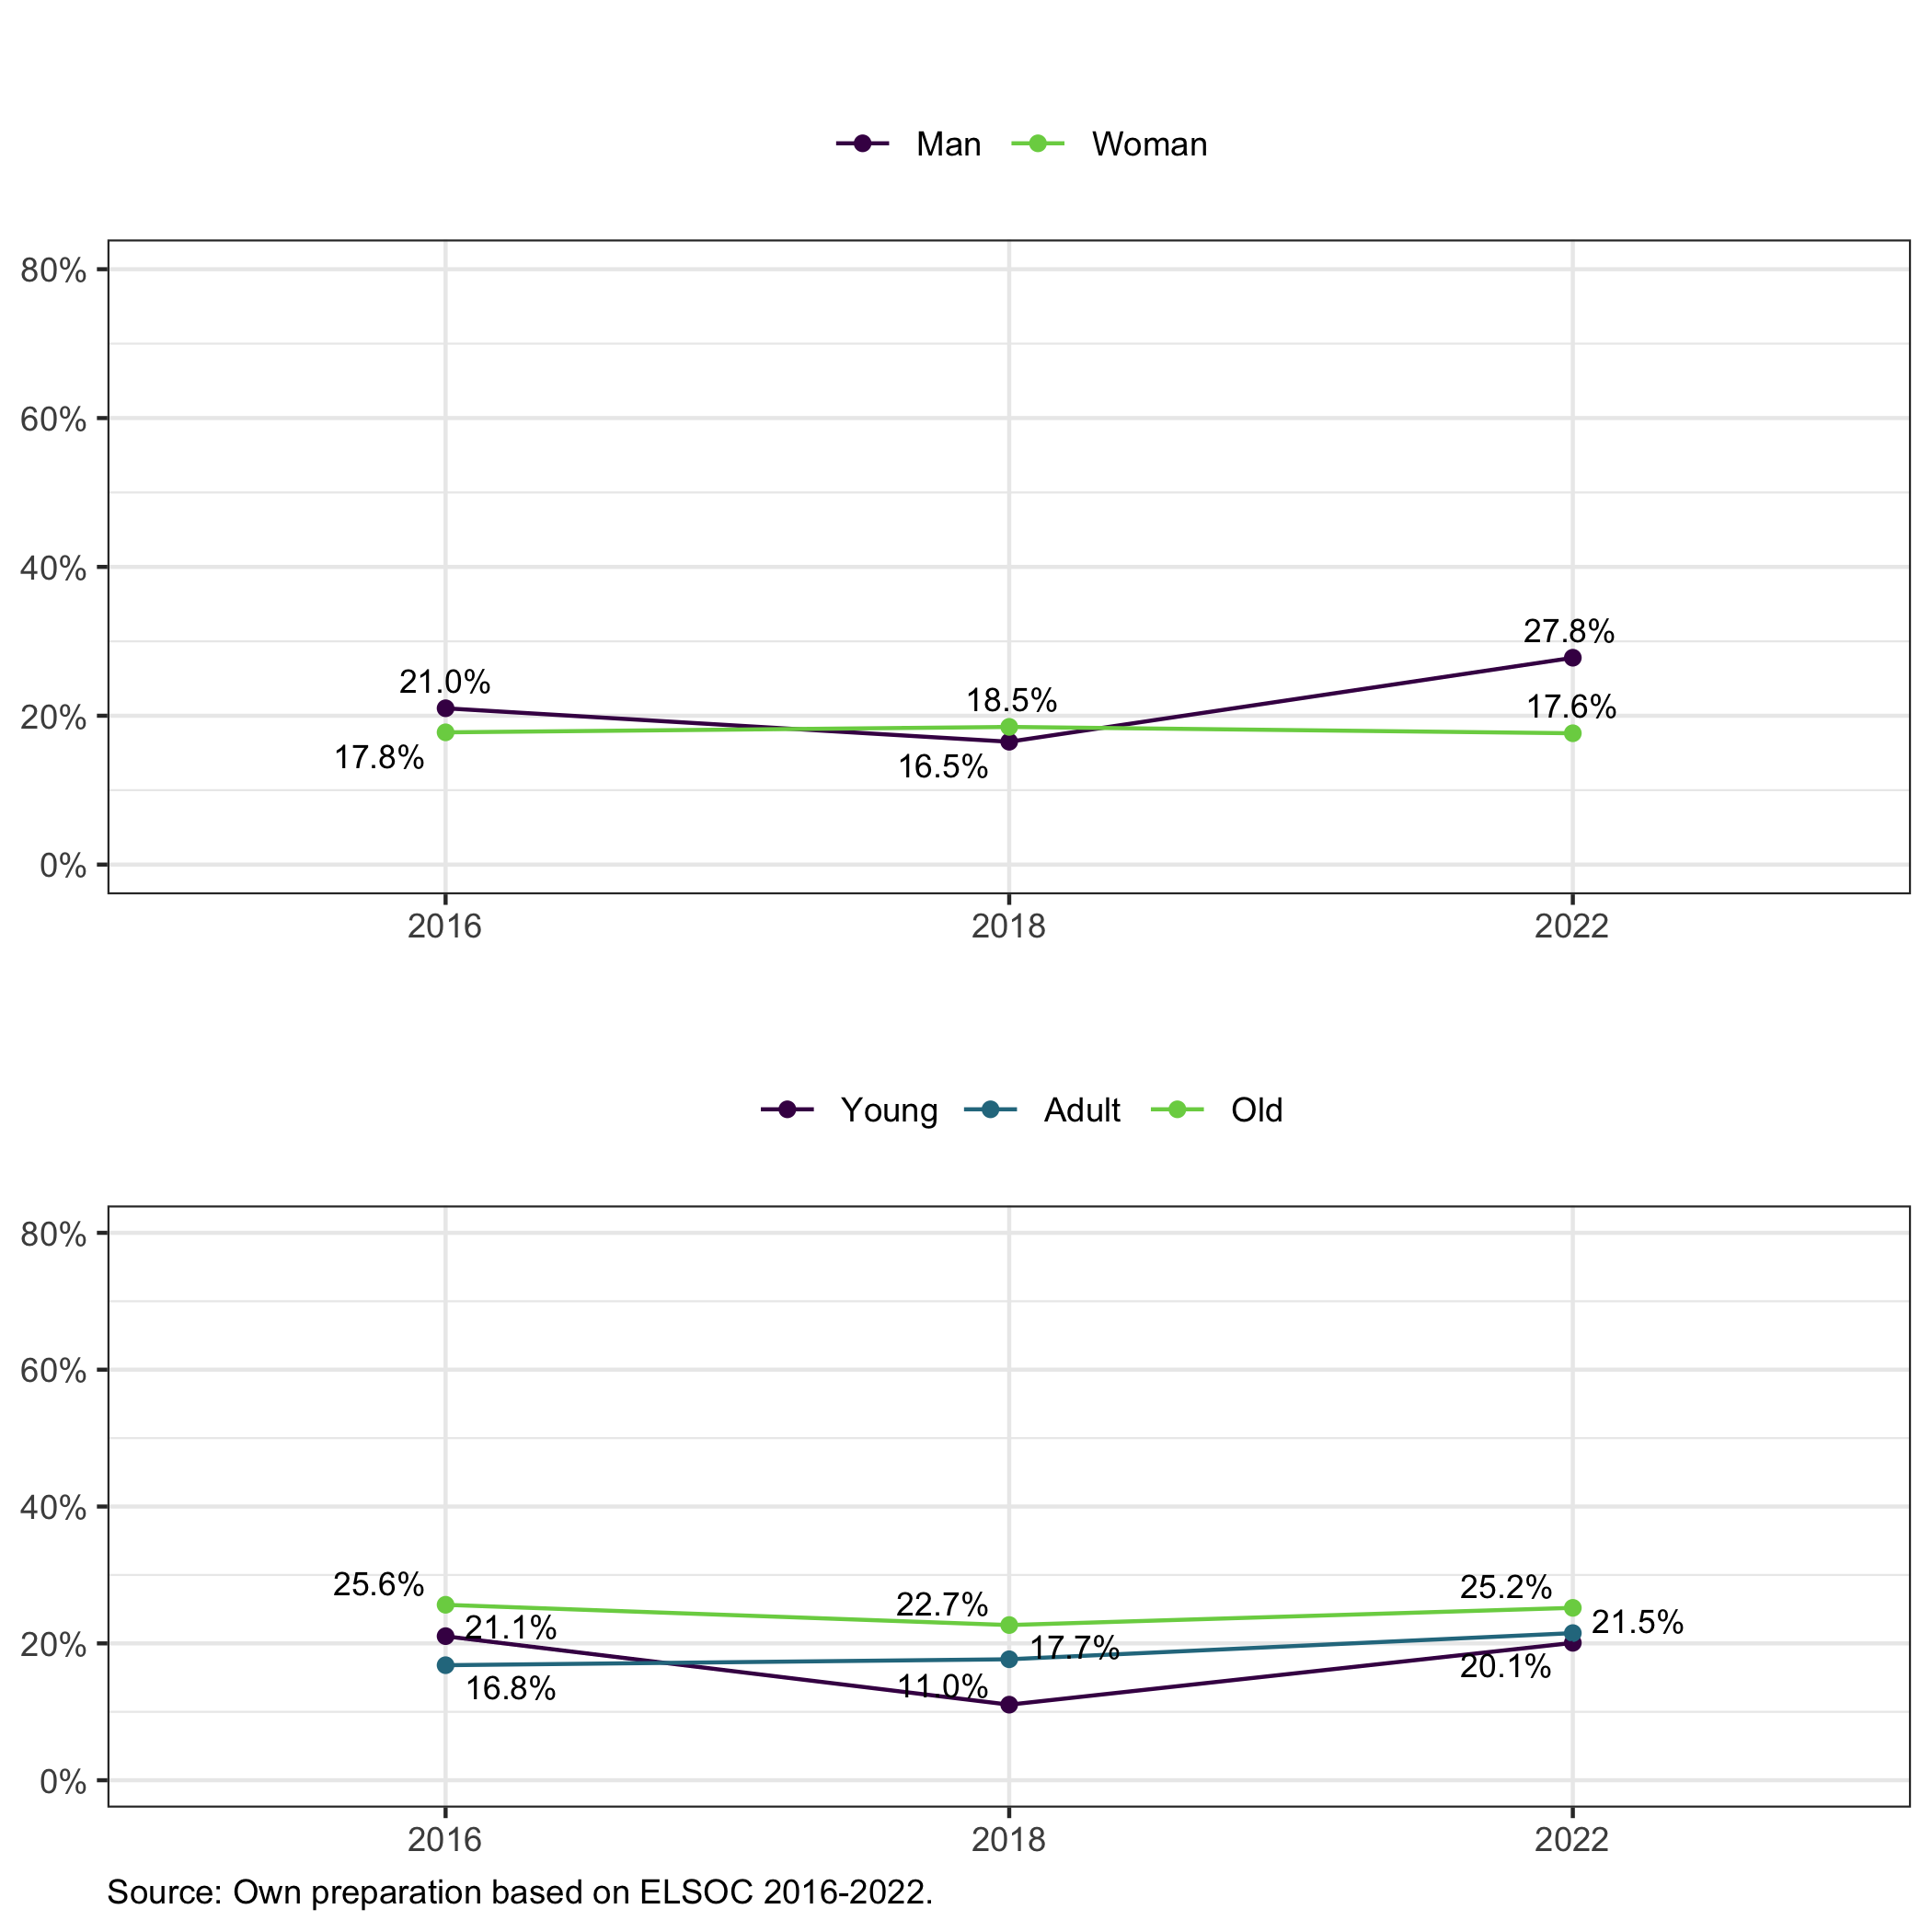
\includegraphics[width=16cm]{output/fig9.png}
    \caption{Active member of two or more organizations}
    \label{fig:fig9}
\end{figure}


\section{Empirical strategy and findings}


\subsection{Latent class analysis}
Longitudinal classification models are based on a first-order homogeneous Markov chain with finite states. The maximum likelihood estimation of the model parameters is performed using the Expectation-Maximization algorithm, computing standard errors through parametric bootstrap. Associational membership indicators serve as response variables ($Y$) to capture manifestations of emerging latent classes. The modeled characteristic of interest is individual associative behavior, unobserved yet evolving across waves:

\begin{equation}
Y= (\text{membership indicators: } association 1,...,association 8)
\end{equation}

These responses feed into the Markov chain model estimating class memberships. Covariates ($X$) are included for explaining the latent distribution, with initial and transition probabilities parameterized using a logit multinomial form, as suggested by Bartolucci \parencite*{bartolucci_latent_2009}:

\begin{equation}
\log\frac{P(U^{1}=u|X^{(1)}=\text{gender, age, education})}{P(U^{1}=1|X^{(1)}=\text{gender, age, education})}=\log\frac{\pi_{u}|x}{\pi_{1}|x}=\beta_{0u}+x^{\top}\beta_{1u}, u=2,...,5
\end{equation}

As discussed previously, this model captures time variation in two main ways: Through the first-order Markov latent process, which allows the probability of a unit being in a certain latent state to change from one time period to the next based on the transition probabilities.
By including covariates that affect the latent Markov process probabilities. This allows systematic time changes related to evolving individual characteristics to be modeled explicitly. Moreover, the model does not impose time homogeneity constraints on the conditional response probabilities given the latent states captured through indicators $Y$. This allows additional temporal heterogeneity in the relationship between the observed responses and latent classes.
\bigskip

In the above expressions, $\beta_u$ and $\gamma_{\overline{u}u}$ are parameter vectors estimated, which are collected in matrices $\beta$ and $\Gamma$. As mentioned by Bartolucci \parencite*{bartolucci_lmest_2017}, when covariates affect the latent process distribution, they are typically excluded from the measurement model, adopting the constraint $\phi^{(t)}{jy|ux}=\phi{jy|u}$.
\bigskip

The latent class analysis allows us to uncover configurations of individuals based on their patterns of multiple memberships in groups or organizations. Ronald Breiger \parencite*{breiger_duality_1974} notes that individuals come together within groups, forming collectivities based on shared interests, affinities or status. At the same time, an individual's specific pattern of affiliations helps define their individuality. There is a duality between the interpersonal and intergroup networks, which our approach bridges by modeling the multiple membership data. The latent classes represent groups of individuals engaged in similar associative behavior, emerging from the complex pattern of multiple memberships. This associative behavior is key to the cohesion and functioning of the overall associative field. The classes and their connections form the backbone of the field's structure.
\bigskip

Moreover, we move beyond static representations to capture dynamic aspects by modeling these latent classes as evolving through a first-order Markov process. The transition probabilities between latent classes from one-time point to the next shed light on the trajectories of groups of individuals with shared associative tendencies. This provides insight not afforded by time-invariant latent class models. Overall, the latent Markov modeling of multiple membership data allows us to analyze the empirical compositions and transformations of the associative field by discerning coherent groups of individuals tied by common affiliations, viewed from a dynamic perspective. 


% latex table generated in R 4.1.2 by xtable 1.8-4 package
% Thu Jun  1 17:43:38 2023
\begin{table}[H]
\centering
\begin{threeparttable}
\caption{\label{demo-table} Fit statistics of class models}
\begin{tabular}{rrrrrr}
  \hline
 & states & lk & np & aic & bic \\ 
  \hline
1 & 1.00 & -14394.87 & 8.00 & 28805.74 & 28848.76 \\ 
  2 & 2.00 & -13586.64 & 46.00 & 27265.28 & 27512.66 \\ 
  3 & 3.00 & -12965.46 & 104.00 & 26138.91 & 26698.20 \\ 
  4 & 4.00 & -12734.50 & 102.00 & 25833.01 & 26811.76 \\ 
  5 & 5.00 & -12523.17 & 200.00 & 25606.33 & 27112.11 \\ 
   \hline
\end{tabular}
\begin{tablenotes}
    \item[1] According to the BIC relative fit statistic, the 3-class model has the best fit.
  \end{tablenotes}
\end{threeparttable}
\end{table}

The models are evaluated considering the BIC relative fit statistic. This statistic is generally preferred to the AIC statistic, and the model with the smaller number represents the best configuration of goodness-of-fit and complexity \parencite{bartolucci_latent_2015}. Based on Table 1, the model corresponding to the minimum BIC is that with k = 3 latent states. 

\begin{figure}[H]
    \centering
    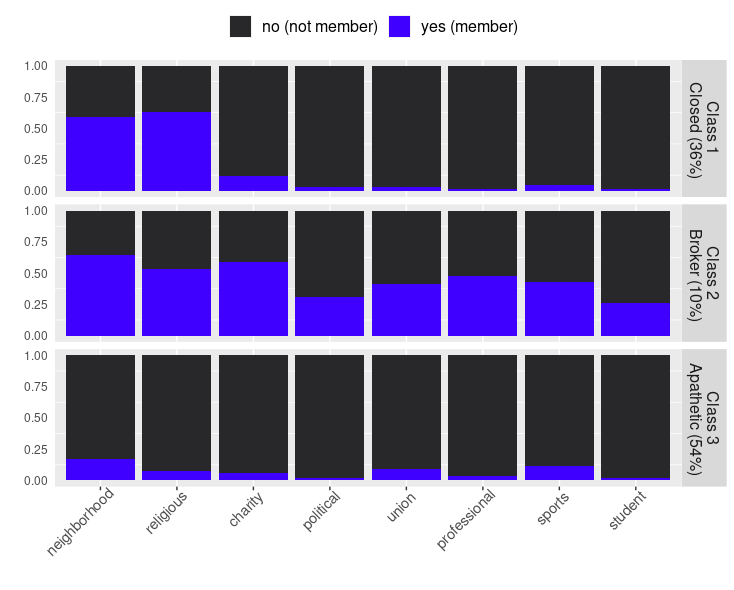
\includegraphics[width=12cm]{output/plot_latentclass2.png}
    \caption{Averaged Initial probabilities.}
    \label{fig:}
\end{figure}


Figure 2 illustrates the summary of averaged conditional probabilities (the estimated conditional response difficulties will be averaged across all observations). We can generally observe that the individuals in the first latent state, which we call "Closed," represent 36 \% of the samples. These individuals present an associative behavior centered on two voluntary associations: neighborhood and religious. A particular aspect of this type of association is that they have solid territorial roots, limiting their ability to influence the local sphere. For its part, the latent state or class two, which we call "brokers," comprises individuals with probabilities of over .1 memberships in all voluntary associations, highlighting the likelihood of being a member of charitable organizations, professionals, and unions. This group and its multiple memberships facilitate articulation, the flow of information, and contagion (e.g., cultural) between different types of associations. This can be considered a structural quality that gives an advantage to individuals while contributing to organizational development and connectivity of the civil society field. Finally, class or state 3 is the majority since it represents 54\% of the sample. We call this class of individuals "apathetic" since they present very low probabilities of participating in associative types. It is worth noting that this pattern of associative behavior has been analyzed and conceptualized as a tendency to withdraw to the private space. For this part, the averaged estimated transition probabilities in the latent class (Markov) model show high persistence in class 1 (apathetic) and class 3 (closed), respectively. Class 2 (broker) is the most fluctuating, with those who go through this "state" or class having a 36\% probability of maintaining this extensive associative behavior. In turn, those in this state have a 25\% chance of going to state 3 (apathetic) and a 39\% chance of going to state 1 (closed). In the annexes section, we illustrate the distribution of marginal probabilities over time. This information shows notable stability for all classes regarding population growth or decline.


\bigskip

\begin{table}[htp]
\centering
\begin{threeparttable}
\caption{\label{demo-table} Multinomial regression}
\begin{tabular}{rrr}
  \hline
 & Class 2 (broker) & Class 3 (apathetic)\\ 
  \hline
Intercept & -1.66** & 1.56*** \\ 
  Mujer & -1.46*** & -1.32*** \\ 
  25-34 & 0.24 & -0.16 \\ 
  35-44 & 0.46 & -0.53 \\ 
  45-54 & 0.47 & -0.70 \\ 
  55-64 & -0.15 & -1.19** \\ 
  65- & -0.67 & -1.72*** \\ 
  Media & 0.82* & 0.49* \\ 
  Técnica & 1.40** & 1.00** \\ 
  Universitaria & 3.24*** & 1.57*** \\ 
   \hline
\multicolumn{3}{l}{\textsuperscript{***}$p<0.01$, 
  \textsuperscript{**}$p<0.05$, 
  \textsuperscript{*}$p<0.1$}
\end{tabular}
\begin{tablenotes}
    \item[1] Class 1 (closed) is reference category.
  \end{tablenotes}
\end{threeparttable}
\end{table}


It is expected that, although this type of behavior can bring benefits at the individual level (greater probability of accessing various resources) and at the social level (social trust), it is difficult to maintain and that there are moments of greater or lesser linkage activity in various groups by individuals, which also depends on the changing needs and purposes of individuals. There are several reasons for this. First, the context does not facilitate associative activity \parencite{oxhorn_neopluralism_2004}. Oxhorn \parencite*{oxhorn_neopluralism_2004} suggests that high levels of inequality and concentration of resources are detrimental to individual abilities to establish and maintain membership in voluntary associations and groups to sustain broad collective action. In individual terms, this suggests that economic insecurity has limited the ability of workers and other economically disadvantaged groups to participate in the public sphere while also eroding their willingness to participate: "The need to survive from day to day can make the public participation and collective action seem, at best, a luxury one can no longer afford and, at worst, wasted effort" (Oxhorn, 2004, p. 302). This may explain not only the low levels of membership reported but also the low probability of maintaining associative behaviors that contribute to the integration of the field through multiple affiliations.


\subsection{Random-effect probit model and findings}
We use random-effect probit model to estimate the relationship between membership in social organizations and social trust for several reasons. First, panel data offers superior capabilities for examining dynamic adjustment processes (Baltagi, 2021). While cross-sectional distribution may appear stable briefly, they obscure numerous underlying changes. For example, in measuring social trust, cross-sectional data can estimate what proportion of the population has a specific level of trust. Repeat cross-sections can show how this proportion changes over time. Second, you can include time-invariant variables (e.g., sex, political affiliation, geographical characteristics) in your model (Baltagi, 2021). In the fixed-effects (Fes) approach, these variables are absorbed by the intercept. Third, FEs estimators of nonlinear models such as binary response models (e.g., probit or logit) suffer from the incidental parameter problem (Cruz-Gonzalez et al., 2017). This makes FEs estimator to be inconsistent. \\

As we mentioned before, the latent class approach allows us to cluster the membership in social organizations and identify three type of classes, such as closed, broker, and apathetic. This classification is our independent variable of interest to understand how associative behavior is related to trust. The following equation represent the empirical model of individual trust:

\begin{equation}
trust_{ijt} = \alpha + \gamma class_{ijt} + \boldsymbol{\beta} \mathbf{X}_{ijt} + Z_{j} + C_{t} + \epsilon_{ijt}
\end{equation}

where the sub index \textit{i} represent the individuals, \textit{j} is used for communes, and \textit{t} represents time (wave $1$, $3$, and $6$). The \textbf{X} vector includes controls for socioeconomic and demographic variable related to our main dependent variable to reduce the bias by omitted these variables are age, sex, marital status, employment status, and a dummy variable for the level of education. The variable $Z$ represents a fixed effect at communal level, which capture some degree of heterogeneity across the space. The variable $C$ is a time fixed effect, a dummy variable for each wave, which captures changes in the time trends. Our main independent variable is $class$, which is a dummy variable that take three values, with a value of one assigned if the individual belongs to class 1 (closed), values of two if she belongs to class 2 (broker), and three if she belongs to class 3 (apathetic). Our primary independent variable is $class$, which is a dummy variable that takes three values, with a value of one assigned if the individual belongs to class 1 (closed), values of two if she belongs to class 2 (broker), and three if she belongs to class 3 (apathetic). Our primary dependent variable is $trust$, a dummy variable that takes a value of one if an individual always trusts others and zero otherwise. Finally, $\epsilon_{ijt}$ is the individual error term. 
\bigskip

We estimate equation (3) using the probit and random-effects probit models (REPM). The advantage of REPM is that it permits analysis at both the individual level and over time. Furthermore, it allows to estimate time-varying and time-invariant covariates in the longitudinal case. REPM considers the positive serial correlation in the error term, while the probit models ignore the correlation, then it is appropriate when the assumptions of homoscedasticity and/or non-correlation of the errors are not valid.
\bigskip

We now turn to the relationship between associative behavior patterns and trust. Table \ref{tab:table5} presents estimates of Equation (3); our baseline specification is based on generalized trust as the dependent variable. The dependent variable in column 1 is generalized trust. We find that individuals belonging to Class 2 (broker) are, on average, $10\%$ more likely to report higher confidence than those belonging to Class 1 (closed). Class 3 (apathetic) is positive and statistically insignificant. Column 3 shows that when we use the REPM, the marginal effects decrease due to autoregressive serial correlation in the error term. The coefficient of Class 2 is significant and positive. It means belonging to Class 2 increases the probability of reporting trusting other people by approximately $4.4\%$ compared to those in Class 1. The dependent variable in columns 1 and 2 is neighborhood trust (NBHD trust); these estimations are statistically insignificant. The above results indicate that associative behavior patterns, measured by the three classes, are linked to a specific type of trust (generalized trust). In practical terms, the estimates indicate that greater exposure to diversity, Class 2, promotes higher levels of generalized trust.


\begin{table}[htbp]\centering
\def\sym#1{\ifmmode^{#1}\else\(^{#1}\)\fi}
\caption{Random effects: marginal effects \label{tab:table5-1}}
\begin{tabular}{l*{4}{D{.}{.}{-1}}}
\hline\hline
            &\multicolumn{2}{c}{Generalized trust}      &\multicolumn{2}{c}{Trust in neighbor}      \\\cmidrule(lr){2-3}\cmidrule(lr){4-5}
            &\multicolumn{1}{c}{Model 1}&\multicolumn{1}{c}{Model 2}&\multicolumn{1}{c}{Model 3}&\multicolumn{1}{c}{Model 4}\\
\hline
Class 1 (closed)&      -0.071\sym{***}&      -0.060\sym{***}&      -0.046         &      -0.073\sym{**} \\
            &     (0.021)         &     (0.020)         &     (0.032)         &     (0.032)         \\
[1em]
Class 3 (apathetic)&      -0.040\sym{*}  &      -0.037\sym{*}  &      -0.091\sym{***}&      -0.092\sym{***}\\
            &     (0.020)         &     (0.020)         &     (0.031)         &     (0.030)         \\
\hline
\(N\)       &        3891         &        3891         &        3891         &        3891         \\
Time Effects&         Yes         &         Yes         &         Yes         &         Yes         \\
Controls    &          No         &         Yes         &          No         &         Yes         \\
\hline\hline
\multicolumn{5}{l}{\footnotesize Standard errors in parentheses}\\
\multicolumn{5}{l}{\footnotesize \sym{*} \(p<0.10\), \sym{**} \(p<0.05\), \sym{***} \(p<0.01\)}\\
\end{tabular}
\end{table}



\begin{figure}[H]
    \centering
    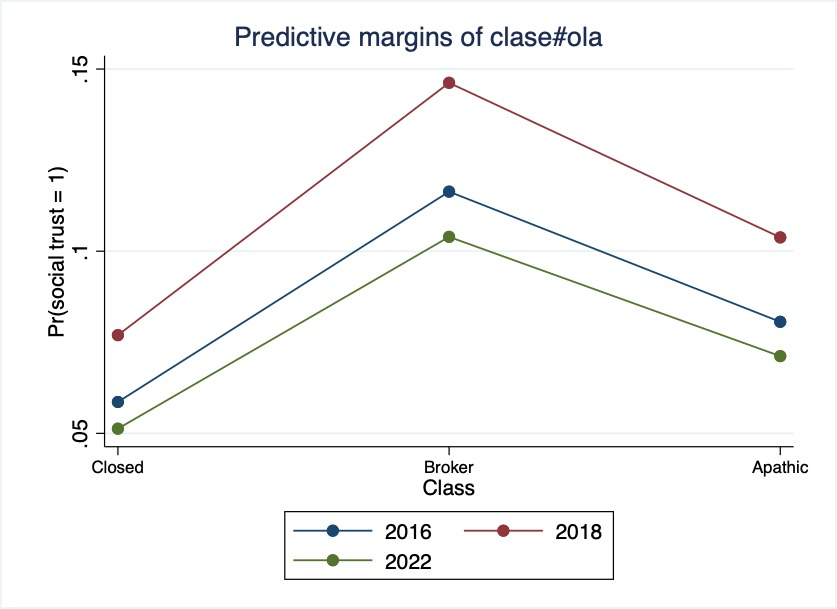
\includegraphics[width=11cm]{output/marginal_effect.jpeg}
    \caption{Active member of two or more organizations}
    \label{fig:fig9}
\end{figure}



\section{Discussion and conclusion}

The intuition that the large-scale patterns of associations in society can tell us something important about the behaviors that dates back at least to Simmel's work on the interconnected web of group affiliations \parencite{centola_how_2018, simmel_conflict_1922}. From here, sociological research has suggested that voluntary associations are focused on collective action that facilitates indirect interaction between individuals who share social attributes and experiences \parencite{mcpherson_hypernetwork_1982}. Therefore, it has been frequently indicated that memberships in voluntary associations can facilitate the interaction of diverse social circles and, in this way, promote social capital development at the individual level \parencite{tindall_network_2012} and integration in complex social systems \parencite{paxton_association_2007}. The argument developed here continues this tradition but emphasizes two things. The first is whether this occurs in the context of high material inequality and social fragmentation. The second is that the connectivity of the associations can be approximated from the behavior patterns detected by observing the multiple affiliations of the individuals. Here, the link between the two associative types is membership shared by organizations, and the connection between individuals is shared membership in a kind of voluntary association. However, we focus on analyzing the associative behavior understood as an individual attribute.
\bigskip

In this paper, we study the relationship between associative behavior patterns and trust in Chile. Our estimation shows that associative behavior patterns are linked to both types of trust. The above finding agrees with Putnam’s hypothesis, which suggests that associative membership is positively associated with generalized trust, suggesting that the more diverse membership patterns facilitate the development of social capital at the individual and collective levels. 
\bigskip

The findings illustrate how diverse associational patterns diffuse generalized trust in high inequality contexts. This form represents abstract willingness to confer confidence toward unfamiliar others based on depersonalized societal appraisals (Paxton 2007). However, territorialized interpersonal trust also matters. Neighborly trust evaluates predictability and cooperation specifically in geographically bounded communities. Despite lacking close ties, familiarity from sharing daily spaces over time allows particularized reputations and expectations among neighbors with weak or indirect links (Consejo Nacional de Participación Ciudadana y Fortalecimiento de la Sociedad Civil 2013). Information diffusion speeds vary between generalized versus localized spheres, enabling contextual interactions. Violations diffusing locally spark targeted sanctions absent in diffuse settings.
\bigskip

While generalized trust facilitates broad cooperation given interdependence with relative strangers, localized trust regulates reciprocity risks among relative familiars. Categorical forms occupy an intermediate zone, ascribing group-based attributes that aid uncertain interactions subsequently updated based on experiences. Together these configurations multidimensionally sustain social integration and civic capital across scales. Specifically, moderate neighborly trust appears to compensate where stranger confidence remains unwillingly low or unrealistically high within a society, preventing extremes through contextual calibration (Paxton 2007). The two display nonlinear linkage, not directly proportional increments. Resonating with the Durkheimian distinction between mechanical and organic solidarity, layers interact dialectically as contemporary complexity obscures direct accountability.
\bigskip

Further exploring contextual complementarities between dual trust spheres can illuminate structural dynamics otherwise masked by conflating levels into singular abstraction. It invites testing especific mechanisms fostering non-zero-sum trusting orientations bridging intimates and strangers. This conceptual refinement also foregrounds open questions on brokerage demands across configurations and socioeconomic asymmetries therein. If diversified associating exhausts, stratification may self-perpetuate despite demonstrating latent connectivity potential. Deepening understandings of layered social trust promises renewed insight on inequality’s erosions of citizenship.
\bigskip




* Observaciones Vicente. 

- La clase de membresías diversas actua como protector de los niveles de confianza social. 
- clases latentes: 
- El efecto se mantiene a nivel local y más general. 
- Establecer la dirección del efecto (va en la dirección Asociatividad y confianza) 
- 

\newpage

\printbibliography

\newpage

\section{Supplementary analysis}

\begin{figure}[H]
    \centering
    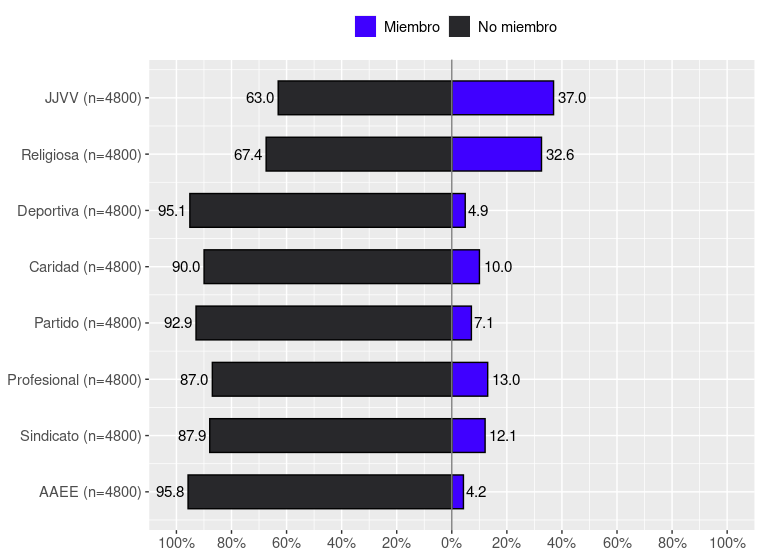
\includegraphics[width=13cm]{output/plot_items.png}
    \caption{Distribución de respuestas para las 3 olas del estudio}
    \label{fig:likert}
\end{figure}


% latex table generated in R 4.1.2 by xtable 1.8-4 package
% Thu Jun  1 19:02:37 2023
\begin{table}[htp]
\centering
\begin{threeparttable}
\caption{\label{demo-table} Multinomial regression}
\begin{tabular}{rrr}
  \hline
 & Class 2 (broker) & Class 3 (apathetic)\\ 
  \hline
Intercept & -1.66** & 1.56*** \\ 
  Mujer & -1.46*** & -1.32*** \\ 
  25-34 & 0.24 & -0.16 \\ 
  35-44 & 0.46 & -0.53 \\ 
  45-54 & 0.47 & -0.70 \\ 
  55-64 & -0.15 & -1.19** \\ 
  65- & -0.67 & -1.72*** \\ 
  Media & 0.82* & 0.49* \\ 
  Técnica & 1.40** & 1.00** \\ 
  Universitaria & 3.24*** & 1.57*** \\ 
   \hline
\multicolumn{3}{l}{\textsuperscript{***}$p<0.01$, 
  \textsuperscript{**}$p<0.05$, 
  \textsuperscript{*}$p<0.1$}
\end{tabular}
\begin{tablenotes}
    \item[1] Class 1 (closed) is reference category.
  \end{tablenotes}
\end{threeparttable}
\end{table}


\begin{figure}[htp]
    \centering
    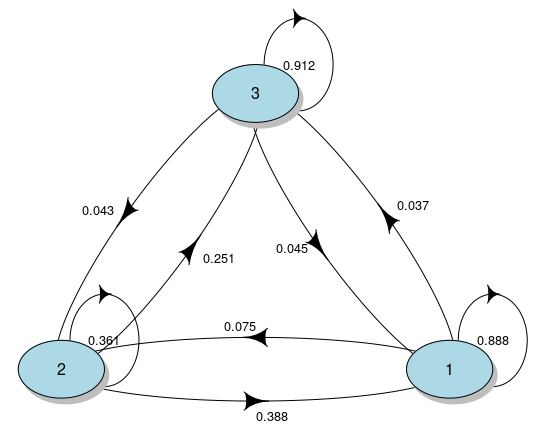
\includegraphics[width=11cm]{output/plot_transition.png}
    \caption{Averaged transition probabilities}
        \label{fig:trans}
\end{figure}

\begin{figure}[htp]
    \centering
    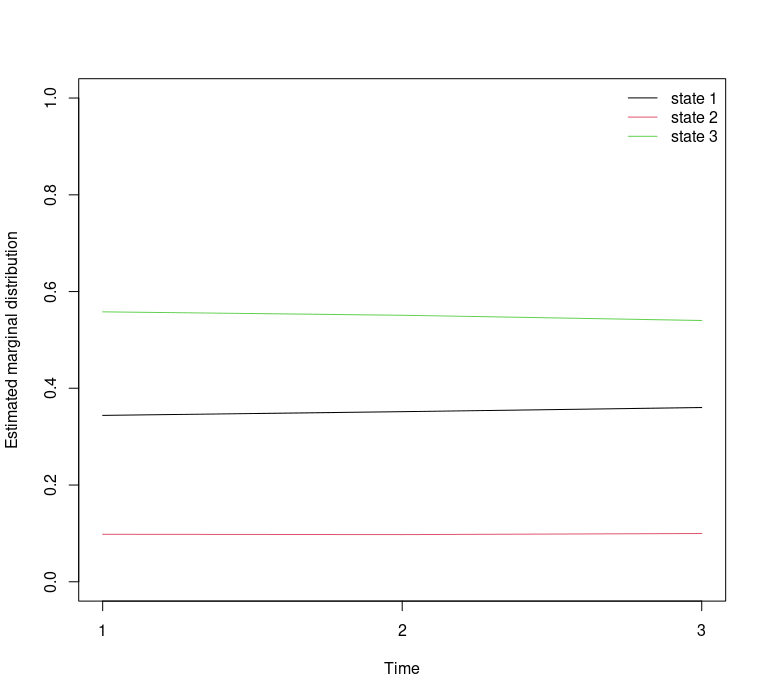
\includegraphics[width=13cm]{output/emd_plot.png}
    \caption{Estimated marginal distribution}
        \label{fig:emd}
\end{figure}


\end{document}
